\section{\texttt{animation}}

%-----------------------------------------------------------------------

\subsection{Descrição}

\begin{frame}

  \begin{quote}
    ``To turn ideas in animations (as quick and faithfully as
    possible).''
  \end{quote}
  \hspace{0.66\linewidth} Yihui Xie \vspace{\baselineskip}

  \texttt{animation} contém funções para produzir animações com o R em
  vários formatos: flash, gif, html, pdf e vídeos.

  \begin{itemize}
  \item Autores: Yihui Xie, Lijia Yu, Weicheng Zhu.
  \item Lançamento: 11-Nov-2007.
  \item Versão: 2.3.
  \item URL:
    \url{http://cran.r-project.org/web/packages/animation/index.html},
    \url{http://yihui.name/animation/}
  \item Third-party software:
    \begin{itemize}
    \item ImageMagik (gif, mpeg convert),
    \item SWF Tools (\texttt{png2swf}, \texttt{jpeg2swf},
      \texttt{pdf2swf})
    \end{itemize}
  \end{itemize}

\end{frame}

%-----------------------------------------------------------------------

\subsection{Como usar}

\frame{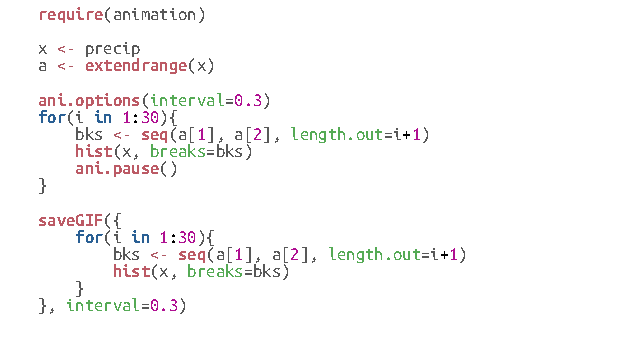
\includegraphics{./tikz/hist_animation-1.pdf}}
\frame{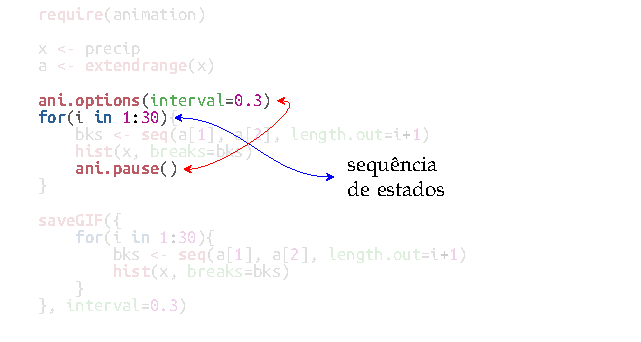
\includegraphics{./tikz/hist_animation-2.pdf}}
\frame{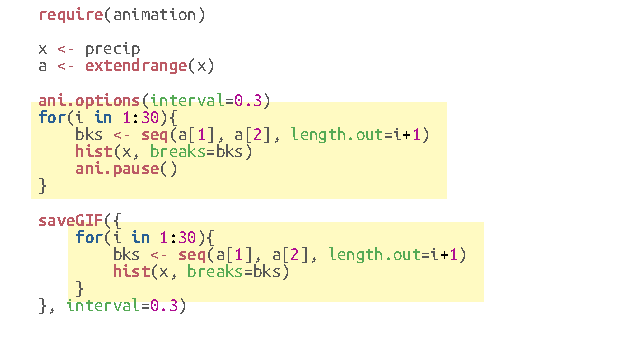
\includegraphics{./tikz/hist_animation-3.pdf}}

%-----------------------------------------------------------------------

\begin{frame}[allowframebreaks]
  \begin{multicols}{2}
    \begin{itemize}
    \item Na janela gráfica
      \begin{itemize}
      \item Mais natural;
      \item Não requer software extra.
      \end{itemize}
    \item HTML
      \begin{itemize}
      \item Não requer software extra, apenas navegador;
      \item Interface de um player de vídeo com botões de play, pause,
        etc;
      \item Não precisa ter o R, pode usar o Rweb.
      \end{itemize}
      \framebreak
    \item GIF
      \begin{itemize}
      \item Requer \texttt{ImageMagick} ou \texttt{GraphicsMagick} para
        converter sequência de imagens em gifs.
      \end{itemize}
    \item Video
      \begin{itemize}
      \item Requer \texttt{FFmpeg} para converter sequência de imagens
        em vídeos.
      \end{itemize}
    \item Flash
      \begin{itemize}
      \item Requer \texttt{SWFTools} para criar animações em flash.
      \end{itemize}
    \end{itemize}
  \end{multicols}
\end{frame}

%-----------------------------------------------------------------------

\subsection{Exemplos}


\begin{frame}

  Praticando:
  \begin{enumerate}
  \item \href{run:../animation/animation.html}{Galeria animation iguir2}
  \end{enumerate}
  
  \vspace{0.5cm} Algumas aplicações com o animation:
  \begin{itemize}
  \item
    \href{http://vis.supstat.com/categories.html\#animation-ref}{Galeria
      do autor}
  \item \href{http://www.r-bloggers.com/?s=animation}{Busca no R
      Bloggers}
  \end{itemize}

\end{frame}
